%%%%%%%%%%%%%%%%%%%%%%%%%%%%%%%%%%%%%%%%%%%%%%%%%%%%%%%%%%%%%%%%%%%%%%%%
% Escuela Politécnica Superior de la Universidad de Alicante
% Realizado por: Jose Manuel Requena Plens
% Contacto: info@jmrplens.com / Telegram:@jmrplens
%%%%%%%%%%%%%%%%%%%%%%%%%%%%%%%%%%%%%%%%%%%%%%%%%%%%%%%%%%%%%%%%%%%%%%%%

\definecolor{mycolor1}{rgb}{1.00000,0.00000,1.00000}%
%
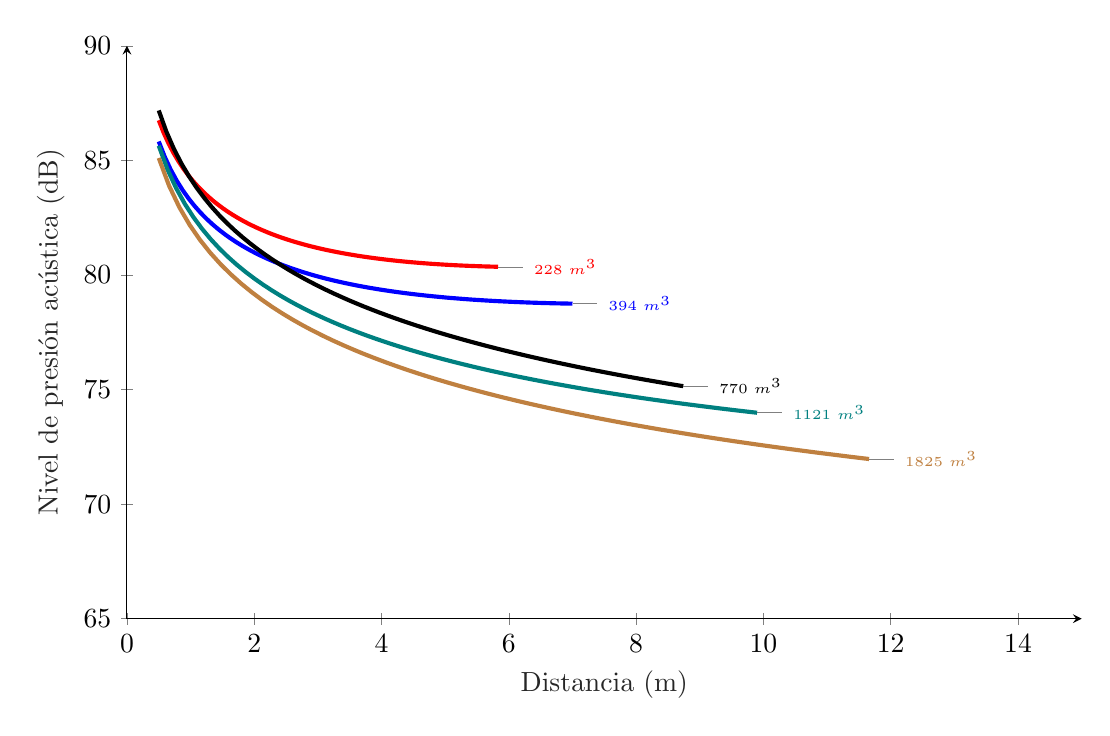
\begin{tikzpicture}

\begin{axis}[%
width=\textwidth,
height=0.6\textwidth,
at={(0\textwidth,0\textwidth)},
scale only axis,
xmin=0,
xmax=15,
xlabel style={font=\color{white!15!black}},
xlabel={Distancia (m)},
ymin=65,
ymax=90,
axis y line=left,
axis x line=bottom,
cycle list name=color list,
ylabel style={font=\color{white!15!black}},
ylabel={Nivel de presión acústica (dB)},
axis background/.style={fill=white},
legend style={legend cell align=left, align=left, draw=white!15!black}
]

% Capos utiles

% 1
\addplot+[ line width=1.5,domain=0.5:5.83, samples=70,every node/.style={xshift=-4pt}]
{10*log10(1.0337e+12 * (  ( 4*0.0026389378 / (272*(-ln(1-0.109))*x) * ( e^(-(13.82*(x/343)*(-3.895) / 1.27))*1.073 - e^(-(13.82*((x/343)+0.05)*1.081 / 1.27))*0.843))))} node [pos=1,pin=0:{\tiny{228 $m^3$}}] {};

% 1.2
\addplot+[ line width=1.5,domain=0.5:7, samples=70,every node/.style={xshift=-4pt}]
{10*log10(1.0337e+12 * (  ( 4*0.0026389378 / (391*(-ln(1-0.109))*x) * ( e^(-(13.82*(x/343)*(-3.646) / 1.40))*1.257 - e^(-(13.82*((x/343)+0.05)*0.921 / 1.40))*0.852))))} node [pos=1,pin=0:{\tiny{394 $m^3$}}] {};

% 1.5
\addplot+[ line width=1.5,domain=0.5:8.74, samples=70,every node/.style={xshift=-4pt}]
{10*log10(1.0337e+12 * ( ( 4*0.0026389378 / (611*(-ln(1-0.109))*x) * ( e^(-(13.82*(x/343)*(-0.123) / 1.76))*2.277 - e^(-(13.82*((x/343)+0.05)*1.047 / 1.76))*0.903))))} node [pos=1,pin=0:{\tiny{770 $m^3$}}] {};

%
%% 1.7
\addplot+[ line width=1.5,color=teal,domain=0.5:9.9, samples=70,every node/.style={xshift=-4pt}]
{10*log10(1.0337e+12 * ( ( 4*0.0026389378 / (785*(-ln(1-0.109))*x) * ( e^(-(13.82*(x/343)*(-0.943) / 1.99))*2.116 - e^(-(13.82*((x/343)+0.05)*1.119 / 1.99))*0.917))))} node [pos=1,pin=0:{\tiny{1121 $m^3$}}] {};

% 20
\addplot+[ line width=1.5,domain=0.5:11.66, samples=70,every node/.style={xshift=-4pt}]
{10*log10(1.0337e+12 * ( ( 4*0.0026389378 / (1086*(-ln(1-0.109))*x) * ( e^(-(13.82*(x/343)*(-0.239) / 2.34))*2.493 - e^(-(13.82*((x/343)+0.05)*1.179 / 2.34))*0.911))))} node [pos=1,pin=0:{\tiny{1825 $m^3$}}] {};

% 20
%\addplot+[ domain=0.5:23.88, samples=70]
%{10*log10(1.0337e+12 * ( ( 4*0.0026389378 / (\S*(-ln(1-0.109))*x) * ( e^(-(13.82*(x/343)*\epsilonE / \T))*\CE - e^(-(13.82*((x/343)+0.05)*\epsilonL / \T))*\CL))))} node [pos=1,pin=0:{\tiny{2431 $m^3$}}] {};

\end{axis}
\end{tikzpicture}%



